\documentclass[a4paper]{article}
\usepackage[14pt]{extsizes} 
\usepackage[T2A]{fontenc}
\usepackage[utf8]{inputenc}
\usepackage{natbib}
\usepackage{graphicx}
\usepackage{amsmath}
\usepackage[english]{babel}
\usepackage{fontspec}
\usepackage{amsmath,amsfonts,amssymb,amsthm,mathtools,mathrsfs}
\usepackage{icomma}
\usepackage{fullpage}
\usepackage{ulem}
\usepackage{eufrak}
\usepackage{setspace}
\usepackage{listings}
\usepackage{indentfirst}
\usepackage[left=2cm,right=1.5cm,top=2cm,bottom=2cm]{geometry}
\usepackage{xcolor}
\usepackage{float}
\usepackage{csquotes}

\setmainfont[Ligatures={TeX,Historic}]{Times New Roman}
\setlength{\parindent}{5ex}
\setlength{\parskip}{1em}
\renewcommand{\baselinestretch}{1}

\graphicspath{{images/}}

\definecolor{buzzlightyear}{HTML}{8757A5}
\definecolor{grass}{HTML}{738D06}
\definecolor{literal}{HTML}{F18A2B}
\definecolor{commentcolor}{HTML}{8E908B}

\lstdefinestyle{habrstyle}{
    backgroundcolor=\color{white},   
    commentstyle=\color{commentcolor},
    keywordstyle=\bfseries\color{buzzlightyear},
    numberstyle=\tiny\color{commentcolor},
    stringstyle=\color{grass},
    basicstyle=\ttfamily\footnotesize,
    breakatwhitespace=false,         
    breaklines=true,                 
    captionpos=b,                    
    keepspaces=true,                 
    numbers=left,                    
    numbersep=5pt,                  
    showspaces=false,                
    showstringspaces=false,
    showtabs=false,                  
    tabsize=4
}

\lstset{style=habrstyle}

\begin{document}

    % FIRST PAGE
    \begin{center}
        \begin{center}
        \hfill \break
        \normalsize{Санкт-Петербургский государственный политехнический}\\
        \normalsize{университет Петра Великого}\\
        \hfill \break
        \normalsize{\textbf{Высшая школа интеллектуальных систем и}}\\ 
        \normalsize{\textbf{суперкомпьютерных технологий}}\\ 
        \hfill \break
        \hfill \break
        \hfill \break
        \normalsize{Лабораторная работа}\\
        \hfill \break
        \hfill \break
        \normalsize{\LARGE Линейные стационарные системы}\\
        \end{center}
        \hfill \break
        \hfill \break
        \hfill \break
        \hfill \break
        \hfill \break
        \hfill \break
        \hfill \break
        \hfill \break
        \hfill \break
        \hfill \break
        \begin{flushright}
            \normalsize{Работу выполнил студент}\\
            \normalsize{3-го курса, группа 3530901/80201}\\
            \normalsize{Сахибгареев Рамис Ринатович}\\
            \hfill \break
            \normalsize{Преподаватель:}\\
            \normalsize{Богач Наталья Владимировна}\\
        \end{flushright}
        \hfill \break
        \hfill \break
        \hfill \break
        \hfill \break
        \begin{center} Санкт-Петербург 2021 \end{center}
        \thispagestyle{empty}
    \end{center}
    % FIRST PAGE [END]
    
    \newpage
        \tableofcontents
    
    \newpage
         \listoffigures
    
    \newpage
         \lstlistoflistings   
     
    % START START START START START
    \newpage
        \section{Part 1: Research and execution of chap010}
        
        In this part we need to research and execute existing chap10.ipynb file, that contains information about stationary systems, impulse response, and convolution theorem. Also we need to perform padding of an violin record with zeros to remove folding effect.
        
        \begin{lstlisting}[language=Python,caption=Padding compare code,label={lst:part1_2}]
    import numpy as np
    import matplotlib as plt
    from thinkdsp import *
    
    response_base = read_wave('180960__kleeb__gunshot.wav')

    start = 0.12
    response = response_base.segment(start=start)
    response.shift(-start)
    
    response.zero_pad(2**17)
    
    response.normalize()
    response.plot()
    decorate(xlabel='Time (s)')
    
    response1 = response_base.segment(start=start, duration=1)
    response1.shift(-start)
    
    response1.normalize()
    
    violin = read_wave('92002__jcveliz__violin-origional.wav')

    start = 0.11
    violin2 = violin.segment(start=start, duration=2)
    violin2.shift(-start)
    
    violin2.truncate(len(response))
    violin2.zero_pad(len(response))
    
    violin2.normalize()
    violin2.plot()
    decorate(xlabel='Time (s)')
    
    start = 0.11
    violin = violin.segment(start=start, duration=2)
    violin.shift(-start)
    violin.truncate(len(response1))
    violin.normalize()
    
    transfer = response.make_spectrum()
    transfer1 = response1.make_spectrum()
    spec1 = violin.make_spectrum()
    spec2 = violin2.make_spectrum()
    print(len(spec1), len(spec2), len(transfer), len(transfer1))
    out1 = (spec1 * transfer1).make_wave()
    out2 = (spec2 * transfer).make_wave()
    out1.normalize()
    out2.normalize()
        \end{lstlisting}
        
        \begin{figure}[H]
            \centering
            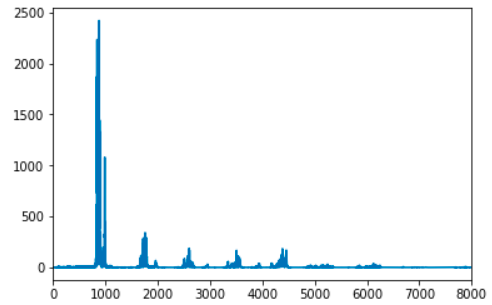
\includegraphics[width=\textwidth]{img/p1_1.png}
            \caption{After padding}
            \label{fig:p1_2}
        \end{figure}
        
        \begin{figure}[H]
            \centering
            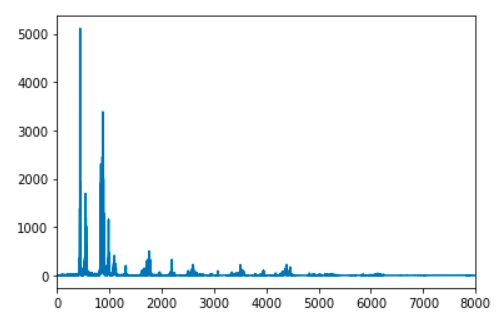
\includegraphics[width=\textwidth]{img/p1_2.png}
            \caption{Without padding}
            \label{fig:p1_2}
        \end{figure}
        
        We can clearly see, that 500 Hz peak disappeared on the record with padding.
        
        \begin{figure}[H]
            \centering
            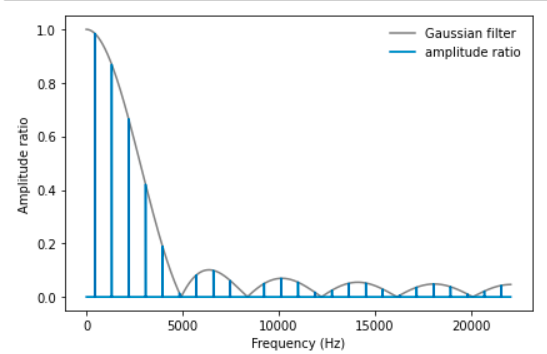
\includegraphics[width=\textwidth]{img/p1_3.png}
            \caption{Trying to apply convolution theorem on non periodic signal}
            \label{fig:p1_1}
        \end{figure}
        
    \newpage
        \section{Part 2: Applying impulse to the signal}

        In this part we need to try to apply an impulse to the signal by ourselves. For the impulse balloon pop sound was used. Let's firstly read it and display its wave. I've extended it with zeros to make folding effect not to appear.
        
        \begin{lstlisting}[language=Python,caption=Reading the impulse,label={lst:part1_2}]
    import numpy as np
    import matplotlib as plt
    from thinkdsp import *
    
    response = read_wave('balloon.wav')
    
    start = 0
    duration = 1
    response = response.segment(duration=duration)
    response.shift(-start)
    
    response.normalize()
    response.unbias()
    response.zero_pad(2**17)
    response.plot()
    decorate(xlabel='Time (s)')
    
    transfer = response.make_spectrum()
    transfer.plot()
    decorate(xlabel='Frequency (Hz)', ylabel='Amplitude')
        \end{lstlisting}
        
        \begin{figure}[H]
            \centering
            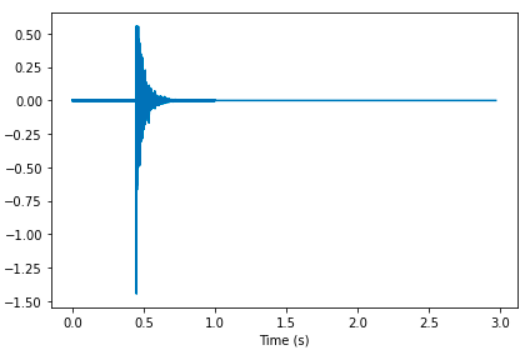
\includegraphics[width=\textwidth]{img/p2_1.png}
            \caption{Impulse's wave}
            \label{fig:part1_1_2}
        \end{figure}
        
        \begin{figure}[H]
            \centering
            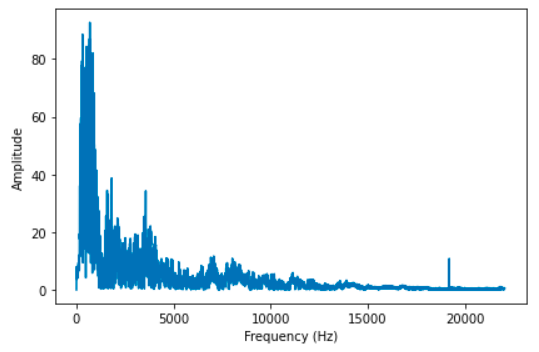
\includegraphics[width=\textwidth]{img/p2_2.png}
            \caption{Impulse's spectrum}
            \label{fig:part1_1_2}
        \end{figure}
        
        Next, let's read the record, that will be affected with the impulse. It is also extended with zeros.
        
        \begin{lstlisting}[language=Python,caption=Reading a violin sound,label={lst:part1_2}]
    wave = read_wave('violin.wav')

    start = 0.12
    wave = wave.segment(start=start, duration=duration * 1.5)
    wave.shift(-start)
    
    wave.truncate(len(response))
    wave.zero_pad(len(response))
    wave.normalize()
    wave.plot()
    decorate(xlabel='Time (s)')
        \end{lstlisting}
        
        \begin{figure}[H]
            \centering
            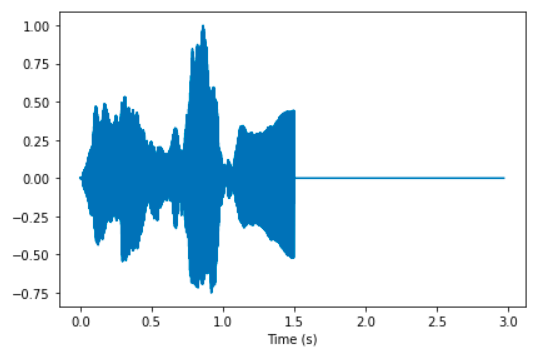
\includegraphics[width=\textwidth]{img/p2_3.png}
            \caption{Violin's wave}
            \label{fig:part1_1_2}
        \end{figure}
        
        Now we can apply the impulse to the violin sound using DFT multiplication.
        
        \begin{lstlisting}[language=Python,caption=Applying the impulse,label={lst:part1_2}]
    output = (wave.make_spectrum() * transfer).make_wave()
    output.normalize()
    output.plot()
        \end{lstlisting}
        
        \begin{figure}[H]
            \centering
            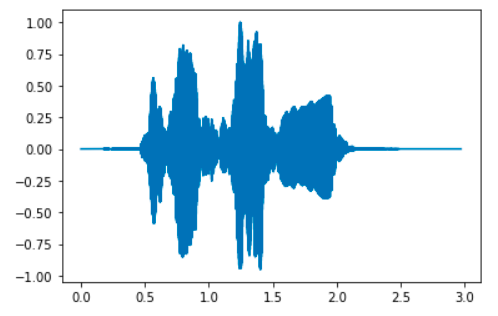
\includegraphics[width=\textwidth]{img/p2_4.png}
            \caption{Impulse applied}
            \label{fig:part1_1_2}
        \end{figure}
        
        Now we can listen the waves and compare them. Also let's compare DFT multiplication to the convolve function.
        
        \begin{figure}[H]
            \centering
            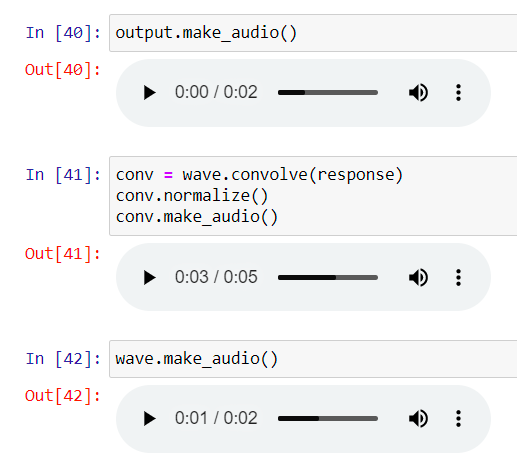
\includegraphics[width=\textwidth]{img/p2_5.png}
            \caption{Comparing results}
            \label{fig:part1_1_2}
        \end{figure}
        
        After listening, no differences between DFT multiplication and convolve method have been found. Also modified sound is more muted, than the original one.
            
    \newpage
        \section{Conclusion}
            We've learned, how we can convert any signal to the impulse and use it as a filter using impulse response. Also we can apply signal using DFT multiplication and convolution. However, we can face the folding effect, but we can easily remove it by extending the signal with zeros. It happens, because real signals are non-periodic, while we are trying to make them periodic.
     
\end{document}
